% main.tex - validacion estatica del modelo extendido DEB (CO2/CH4, H. illucens)
% Compilar: xelatex main; biber main; xelatex main; xelatex main
\documentclass[11pt,a4paper]{article}

\usepackage{fontspec}
\setmainfont{TeX Gyre Termes}
\setsansfont{TeX Gyre Heros}
\setmonofont{Latin Modern Mono Light}

\usepackage[spanish,es-noquoting]{babel}
\usepackage{amsmath}
\usepackage[margin=2.5cm]{geometry}
\usepackage{graphicx}
\usepackage{booktabs}
\usepackage{siunitx}
\usepackage{caption}
\usepackage{tikz}

\usepackage[backend=biber,style=authoryear,sorting=nyt]{biblatex}
\addbibresource{bibliografia/bibliografia.bib}

\usepackage[hidelinks]{hyperref}

\title{Modelado y validación experimental de emisiones de CO$_2$
  con separación de fuentes larvaria y microbiana en bioconversión
  estática con \textit{Hermetia illucens}}
\author{%
\begin{tabular}{cc}
John Jairo Leal Gómez${}^{1}$ & Sorany Milena Barrientos${}^{2}$\\[2pt]
Luis Octavio González${}^{1}$ & Luis Fernando Mejía${}^{1}$
\end{tabular}\\[8pt]
{\small ${}^{1}$Facultad de Ingeniería y Administración}\\
{\small ${}^{2}$Facultad de Ciencias Agropecuarias}\\
{\small Universidad Nacional de Colombia, Sede Palmira, Valle del Cauca, Colombia}
}
\date{\today}

\begin{document}
\maketitle

\begin{abstract}
\noindent La bioconversión con larvas de \textit{Hermetia illucens} valoriza residuos orgánicos, pero emite gases de efecto invernadero cuyas fuentes (respiración larvaria y degradación microbiana del lecho) no se han separado experimentalmente en los modelos disponibles. Este trabajo valida un modelo dinámico de emisiones de CO$_2$ construido como extensión del modelo DEB de Eriksen, con tres componentes nuevos: un interruptor de prepupa que cierra la asimilación, un módulo microbiano del lecho y el balance de gas de la cámara estática. El experimento por lotes sellado incluyó dos dietas (alimento estándar y residuos agroindustriales de frutas fermentados), cierres por triplicado (réplicas técnicas), controles de alimento solo y sensores de CO$_2$ y CH$_4$, y la validación explotó la descomposición de fuentes (tratamiento menos control). La componente larvaria reprodujo las tasas netas dentro de la incertidumbre experimental ($R^2 = 0.981$, RMSE de 5.2 ppm/min en la dieta de residuos; en la dieta estándar el colapso de las emisiones se atribuye al agotamiento del sustrato, con una cota inferior incumplida) y el interruptor de prepupa resultó esencial para capturar el colapso de las emisiones al final del ciclo en la dieta de residuos. Usando solo mediciones de gas, el ajuste cuantificó la calidad relativa de la dieta de residuos (70 \% de la estándar), los tiempos de prepupa (12.1 a 16.4 días) y los parámetros microbianos ($k_{\mathrm{ref}} \approx 0.28$ a $0.29$ d$^{-1}$, $Y_{CO_2} \approx 1.13$ a $1.39$); el CH$_4$ se reportó como indicador cualitativo. Como prueba de concepto con un lote por dieta y réplicas técnicas, el modelo y el protocolo de validación son una base para el diseño de dietas y la operación del proceso, y son transferibles a otros insectos de bioconversión.

\vspace{6pt}
\noindent\textbf{Palabras clave:} \textit{Hermetia illucens}; bioconversión; emisiones de CO$_2$; modelo DEB; cámara estática; validación por fuentes.
\end{abstract}

\section{Introduccion}
\label{sec:introduccion}

Los residuos organicos representan una fraccion mayoritaria de los desechos municipales y agroindustriales, y su disposicion en vertederos es una fuente importante de emisiones de gases de efecto invernadero (GEI). La bioconversion con larvas de la mosca soldado negra (\textit{Hermetia illucens}) se ha consolidado como una alternativa de valorizacion: las larvas transforman residuos en biomasa rica en proteina y lipidos, con alta reduccion de masa y humedad del sustrato \parencite{mertenatBlackSoldierFly2019,nayakHermetiaIllucensDiptera2023}. Sin embargo, el proceso no esta exento de emisiones: la respiracion larvaria y la degradacion microbiana del lecho liberan CO$_2$, y bajo ciertas condiciones del sustrato se han reportado emisiones de CH$_4$ y N$_2$O \parencite{ermolaevGreenhouseGasEmissions2019,parodiBioconversionEfficienciesGreenhouse2020a,boakye-yiadomGreenhouseGasEmissions2022,lindbergProcessEfficiencyGreenhouse2022a}.

La cuantificacion de estas emisiones se ha hecho tipicamente con camaras estaticas o sistemas de flujo, siguiendo metodos establecidos \parencite{hutchinsonMethodsSoilAnalysis1992}, y muestra una fuerte dependencia del sustrato y las condiciones del proceso \parencite{parodiBioconversionEfficienciesGreenhouse2020a,boakye-yiadomGreenhouseGasEmissions2022}. Mas recientemente, los sensores de bajo costo han permitido el monitoreo continuo de CO$_2$ y CH$_4$ en estos sistemas \parencite{mitchellCalibrationLowCostMethane2024,kiplimoAddressingLowCostMethane2024}. No obstante, las mediciones reportan emisiones totales del sistema larvas--lecho, sin separar la contribucion de cada fuente, lo que limita su utilidad para el diseno de dietas y la operacion del proceso.

En paralelo, la modelacion matematica de la bioconversion ha avanzado hacia modelos dinamicos mecanicistas. Sobre la base de la teoria de presupuestos dinamicos de energia (DEB) \parencite{kooijmanDynamicEnergyBudget2009}, \textcite{eriksenDynamicModellingFeed2022} propuso un modelo de compartimentos que describe la asimilacion del alimento, el crecimiento estructural, la acumulacion de lipidos y la produccion de CO$_2$ de larvas de \textit{H. illucens}, luego aplicado al desempeno metabolico bajo restriccion alimentaria \parencite{eriksenMetabolicPerformanceFeed2024}. Otros trabajos han modelado el crecimiento larvario \parencite{padmanabhaComprehensiveDynamicGrowth2020}, el desempeno por dieta \parencite{laganaroGrowthMetabolicPerformance2021a}, el efecto de la temperatura \parencite{schonEffectTemperatureGrowth2024} y la estimacion de las dinamicas de GEI \parencite{rossiEstimatingDynamicsGreenhouse2024a}. A pesar de estos avances, persisten tres vacios: (i) los modelos no se han validado contra mediciones de gas que separen la fuente larvaria de la microbiana; (ii) no representan la transicion a prepupa, en la que la larva deja de alimentarse y las emisiones colapsan, aunque esta domina el final del ciclo productivo; y (iii) al omitir la degradacion microbiana del lecho, no pueden reproducir las emisiones totales medidas en un reactor por lotes.

El objetivo de este artículo es modelar y validar experimentalmente las emisiones de CO$_2$ en la bioconversion estatica con \textit{H. illucens}, distinguiendo lo que generan las larvas de lo que genera la degradacion microbiana del lecho, con un modelo construido como extension del modelo DEB de \textcite{eriksenDynamicModellingFeed2022,eriksenMetabolicPerformanceFeed2024} con tres componentes nuevos: un interruptor de prepupa que cierra la asimilacion, un modulo microbiano del lecho con un estado de biomasa cuya degradacion es de primer orden en la biomasa, limitada por el sustrato y modulada por humedad y temperatura, y el balance de gas de la camara estatica que conecta las fuentes con la medicion. La validacion explota la descomposicion de fuentes: la componente larvaria se contrasta con la tasa neta (tratamiento menos control de alimento solo) y la microbiana con los controles, en un experimento por lotes sellado con dos dietas (alimento estandar y residuos agroindustriales de frutas fermentados), cierres por triplicado (replicas tecnicas) y sensores de CO$_2$ y CH$_4$; las lecturas de CH$_4$ se usan solo como indicador cualitativo por la falta de calibracion del sensor. El articulo se organiza asi: la seccion 2 describe el sistema experimental, el modelo extendido, su solucion numerica y el analisis de incertidumbre; la seccion 3 presenta la calibracion y la validacion; la seccion 4 discute los alcances y limitaciones; y la seccion 5 concluye.

% secciones/métodos.tex
\section{Materiales y métodos}
\label{sec:metodos}

\subsection{Sistema experimental y protocolo de medición}
\label{sec:sistema}

Los experimentos se realizaron en recipientes plásticos rígidos de geometría
troncopiramidal rectangular: boca superior de $37 \times 26$~cm, base de
$32 \times 21$~cm y altura de $17$~cm, para un volumen geométrico de
$\approx 13{,}8$~L. Los sensores de gases (CO$_2$, MH-410D; CH$_4$, MH-440D)
se montaron empotrados en una de las caras laterales mayores, con el elemento
sensible hacia el interior y por encima del nivel del sustrato. Durante cada
cierre el recipiente se mantuvo sellado con su tapa reforzada con silicona, y
el volumen de aire efectivo $V_{\mathrm{aire}}$ ---el volumen geométrico menos
el ocupado por el recipiente interno y su contenido--- entró como parámetro
medido en el cálculo de tasas.

El sustrato y las larvas se alojaron en un recipiente plástico de
$15 \times 12 \times 5$~cm con tapa aireada por malla, colocado dentro de la
cámara; se supuso equilibrio rápido de gases entre el recipiente interno y el
aire de la cámara a través de la malla. El mismo tipo de montaje se usó en
tratamientos y controles, de modo que $V_{\mathrm{aire}}$ fue comparable entre
ellos.

Se evaluaron dos dietas, D1 y D4, cuya composición se detalla en la
Cuadro~\ref{tab:dietas}. En cada día de medición los cierres se realizaron de
forma secuencial por dieta: primero un recipiente hasta la saturación del
sensor de CO$_2$ (6000~ppm) y luego el otro, con el mismo procedimiento. Cada
condición se midió con tres cierres consecutivos sobre el mismo lote (réplicas técnicas de medición); el valor reportado por punto es su media y el rango su dispersión. Las réplicas biológicas (lotes independientes) quedan como extensión futura. Como controles se incluyeron
recipientes con alimento solo (respiración del sustrato) y con larvas solas
(mantenimiento sin alimento), medidos con el mismo protocolo; la tasa neta de
cada tratamiento se obtuvo restando el control correspondiente del mismo día.

Cada lote se cargó una sola vez al inicio del ciclo, sin reposición ni
retiro: 250~g de sustrato por recipiente, preparado mezclando el
alimento seco con agua hasta una humedad del 70~\% en base húmeda
(75~g de materia seca y 175~g de agua), y 700 larvas por tratamiento.
Los controles de alimento solo llevaron los mismos 250~g de sustrato
sin larvas. La temperatura dentro de la cámara se registró de forma
continua y se mantuvo aproximadamente constante entre cierres.

La tasa de cada cierre se estimó por ajuste lineal del tramo previo a la
saturación; cuando el ajuste fue de baja calidad o la curva alcanzó el techo
del sensor (cierres marcados como saturados), la tasa estimada es conservadora
y se trató como cota inferior en la validación (sec. \ref{sec:resultados}).

\begin{table}[htbp]
  \centering
  \caption{Descripción de las dietas evaluadas.}
  \label{tab:dietas}
  \begin{tabular}{lp{8cm}}
    \hline
    Dieta & Descripción \\
    \hline
    D1 & Alimento comercial estándar para pollo de engorde (dieta de
         referencia del modelo de Eriksen) \\
    D4 & Residuos agroindustriales de frutas (naranja, plátano, entre
         otras), fermentados \\
    \hline
  \end{tabular}
\end{table}

\subsection{Modelo dinámico del proceso}
\label{sec:modelo}

El proceso se describe con un modelo dinámico de parámetros concentrados (0D) que amplia el modelo de asimilación, crecimiento y producción de CO$_2$ de \textcite{eriksenDynamicModellingFeed2022,eriksenMetabolicPerformanceFeed2024} (en adelante, el \emph{modelo de referencia}) ---desarrollado para larvas de \textit{H. illucens} sobre dieta estándar--- con tres componentes adicionales: (i) un interruptor de prepupa que representa la cesación de la alimentación al final del ciclo larvario; (ii) un módulo microbiano de primer orden para la degradación del sustrato no consumido \parencite{roels1980}; y (iii) un balance de masa de gas en la cabeza de aire de la cámara estática de medición. Los fundamentos de la teoría DEB del núcleo larvario se encuentran en \parencite{kooijmanDynamicEnergyBudget2009,jagerDEBkissQuestSimplest2013}. El modelo supone temperatura constante (medida) y humedad del lecho como variable de estado, oxígeno no limitante dentro de los cierres y número de larvas $N$ constante (mortalidad despreciable en el periodo experimental).

El vector de estado es $\mathbf{x} = (A, B, L, D_M, W, X, c_{CO_2}, c_{CH_4})$, donde $A$, $B$ y $L$ son los compartimentos larvarios (asimilado, estructura y lípidos, mg/larva), $D_M$, $W$ y $X$ la materia seca, el agua y la biomasa microbiana del lecho (g), y $c_i$ las concentraciones de gas en la cabeza de aire (mol/m$^3$). Las condiciones iniciales $A_0 = 0.005$ y $L_0 = 0.003$~mg corresponden a una larva neonata \parencite{eriksenDynamicModellingFeed2022}; $B_0$ se calibró en este trabajo con las tasas netas (Cuadro~\ref{tab:parametros}).

\subsubsection{Núcleo larvario (DEB de Eriksen)}

El núcleo sigue el modelo de compartimentos de \textcite{eriksenDynamicModellingFeed2022}: el alimento asimilado entra al compartimento $A$ y de allí se reparte entre crecimiento estructural $B$, reservas lipídicas $L$ y costos metabólicos pagados como CO$_2$ (Figura \ref{fig:nucleo}); los fundamentos DEB de esta partición están en \parencite{kooijmanDynamicEnergyBudget2009}. A continuación se indica la procedencia de cada expresión.

\begin{figure}[htbp]
\centering
\begin{tikzpicture}[
  comp/.style={draw, rounded corners=2mm, minimum width=3.0cm, minimum height=1.1cm, align=center, fill=gray!8},
  gas/.style={draw, dashed, rounded corners=2mm, minimum width=2.0cm, minimum height=1.1cm, align=center},
  gate/.style={circle, draw, thick, fill=white, inner sep=1.8pt, font=\footnotesize},
  flujo/.style={->, >=latex, thick, shorten >=3pt, shorten <=3pt},
  etiqueta/.style={fill=white, inner sep=1.5pt, font=\footnotesize}]
\node[comp] (alim) at (0,0) {Lecho\\ (alimento)};
\node[comp] (A) at (6.0,0) {$A$: asimilado};
\node[comp] (B) at (11.6,0) {$B$: estructura};
\node[comp] (L) at (11.6,-4.0) {$L$: lípidos};
\node[gas] (CO2) at (6.0,-4.0) {CO$_2$};
\draw[flujo] (alim) -- node[etiqueta, above=2pt]{$r_A$}
                      node[gate, below=2pt]{$S$} (A);
\draw[flujo] (A) -- node[etiqueta, above=2pt]{$(1 + Y_B)\,r_B$} (B);
\draw[flujo] (A) -- node[etiqueta, right=2pt]{$r_{Cm} + Y_B\,r_B$} (CO2);
\draw[flujo] (A.south east) -- node[etiqueta]{$r_L$} (L.north west);
\draw[flujo] (L) -- node[etiqueta, below=2pt]{$Y_L\,r_L$} (CO2);
\end{tikzpicture}
\caption{Compartimentos y flujos de carbono del núcleo larvario (adaptado de \parencite{eriksenDynamicModellingFeed2022}). El interruptor de prepupa $S(t)$ (ecuación \ref{eq:prepupa}) cierra la entrada de alimento al final del ciclo; los costos $r_{Cm}$, $Y_B r_B$ y $Y_L r_L$ salen del sistema como CO$_2$.}
\label{fig:nucleo}
\end{figure}

\paragraph{Interruptor de prepupa (extensión respecto al modelo de referencia).}
Al final del último instar, las larvas de \textit{H. illucens} cesan la
alimentación y entran en prepupa, un estadio de transición a la metamorfosis
en el que el insecto no se alimenta y sostiene su metabolismo con las reservas
acumuladas durante la fase larvaria, principalmente los lípidos del cuerpo
graso \parencite{arreseInsectFatBody2010,nayakHermetiaIllucensDiptera2023}.
Fisiológicamente, la transición es un umbral del ciclo de vida: en los modelos
DEB de insectos holometábolos, los cambios de estadio separan regímenes
energéticos distintos, con asimilación en la fase larvaria y metabolismo de
mantenimiento sobre reservas en las fases no alimentarias
\parencite{kooijmanDynamicEnergyBudget2009,llandresDynamicEnergyBudget2015}.
El modelo de \textcite{eriksenDynamicModellingFeed2022} no incluye este
cierre, por lo que predice asimilación y producción de CO$_2$ sostenidas al
final del ciclo, en contradicción con el colapso de las emisiones observado
entre los días 13 y 17 (sec. \ref{sec:resultados}).

Para representarlo, se introduce la fracción de la cohorte que sigue
alimentándose como una función del tiempo. La forma no es arbitraria: en una
cohorte de $N \approx 700$ larvas la entrada a prepupa no es sincrónica, y si
los tiempos individuales de transición se distribuyen alrededor de un día
central $t_p$ con dispersión $w_p$, la fracción de larvas aún en alimentación
es la función de supervivencia de esa distribución. Para una distribución
logística de los tiempos de transición, dicha fracción es
\begin{equation}
S(t) = \frac{1}{1 + \exp(-(t - t_p)/w_p)},
\label{eq:prepupa}
\end{equation}
con $S \to 1$ al inicio del ciclo (toda la cohorte alimentándose) y $S \to 0$
al final (toda la cohorte en prepupa). El parámetro $t_p$ es el día central de
la transición y $w_p$ su anchura, interpretable como la sincronía de la
cohorte: el límite $w_p \to 0$ corresponde a una transición perfectamente
sincrónica (un interruptor ideal), que sería discontinuo, no estimable con
mediciones diarias y numéricamente rígido; la versión suave es diferenciable y
monótona decreciente, lo que mantiene el campo vectorial continuo para la
integración (sec. 2.3). En el modelo, el factor $(1 - S(t))$ cierra la
asimilación (ec. \ref{eq:asimilacion}) y el suelo de mantenimiento
$m_{\mathrm{suelo}}$ representa el metabolismo residual sobre reservas durante
la prepupa, anclado a la medición de larvas en ayuno (sec. 3). Los parámetros
$t_p$ y $w_p$ se ajustan al descenso de las tasas medidas entre los días 13 y
17.

\paragraph{Asimilación (ecs. 4 y 5 de Eriksen, 2022).}
La tasa específica de asimilación decrece con el tamano y el flujo asimilado es proporcional a $B$ \parencite{eriksenDynamicModellingFeed2022}:
\begin{equation}
a(B, t, D_M) = f\,a_{\max}\,\frac{1}{1 + (B/B_{\max})^{\alpha}}\,(1 - S(t))\,\frac{D_M}{D_M + K_s},
\qquad r_A = a\,B,
\label{eq:asimilacion}
\end{equation}
donde $B_{\max}$ es la biomasa de referencia y $\alpha$ controla la caida con el tamano. El factor $(1 - S(t))$ es el interruptor de prepupa de la ec. \ref{eq:prepupa}: cierra la asimilación al final del ciclo. También son extensiones respecto al modelo de referencia el factor de calidad de dieta $f$ ($f = 1$ en D1, calibrado en D4, sec. \ref{sec:resultados}) y la limitación por disponibilidad de alimento $D_M/(D_M + K_s)$, con $K_s = 2$~g fijo, que apaga la asimilación suavemente cuando el sustrato se agota en el régimen de carga única.

\paragraph{Crecimiento (ec. 10 de Eriksen, 2022).}
El crecimiento estructural sigue la forma logistica con descuento de mantenimiento de \textcite{eriksenDynamicModellingFeed2022}:
\begin{equation}
G(B) = \max\!\left(1 - (B/B_{\max})^{\beta}, 0\right),
\qquad
\mu_B = \max\!\left(\frac{(a - m)\,G}{1 + Y_B\,G}, 0\right),
\qquad r_B = \mu_B\,B,
\label{eq:crecimiento}
\end{equation}
donde $m$ es la tasa de mantenimiento específico, en la tradición de Pirt y los principios macroscopicos de \textcite{roels1980}, y $Y_B$ el costo de crecimiento.

\paragraph{Mantenimiento (Eriksen, 2022, con suelo de prepupa).}
El costo de mantenimiento es proporcional a la estructura, y durante la prepupa cae a un suelo añadido en este trabajo, anclado a la medición de larvas en ayuno del día 17 (sec. \ref{sec:resultados}):
\begin{equation}
r_{Cm} = m\,B\,\big[(1 - S(t)) + m_{\mathrm{suelo}}\,S(t)\big].
\label{eq:mantenimiento}
\end{equation}

\paragraph{Balance de lípidos y CO$_2$ (ec. 12 de Eriksen, 2022).}
Suponiendo el compartimento $A$ en cuasi-equilibrio ($dA/dt \approx 0$), lo asimilado se reparte instantaneamente entre crecimiento, mantenimiento y reservas, lo que da el flujo neto a lípidos y la producción larvaria de CO$_2$ como la suma de los tres costos respiratorios \parencite{eriksenDynamicModellingFeed2022,eriksenMetabolicPerformanceFeed2024}:
\begin{equation}
r_L = r_A - (1 + Y_B)\,r_B - r_{Cm},
\qquad
r_{CO_2}^{\mathrm{lar}} = r_{Cm} + Y_B\,r_B + Y_L\,\max(r_L, 0),
\label{eq:co2lar}
\end{equation}
con $Y_L$ el costo de depósito de lípidos; todas las tasas en mg/larva/d.

\subsubsection{Módulo microbiano del lecho}
En la bioconversión, las larvas no consumen la totalidad del sustrato: la
fracción no asimilada permanece en el lecho, donde es descompuesta por la
microbiota ambiental en paralelo al consumo larvario (Figura
\ref{fig:lecho}). Esta fuente no es despreciable: las emisiones medidas en
reactores con \textit{H. illucens} mezclan la respiración larvaria y la
microbiana \parencite{ermolaevGreenhouseGasEmissions2019,parodiBioconversionEfficienciesGreenhouse2020a},
y en los controles de alimento solo de este experimento las tasas de CO$_2$
aumentaron de forma sostenida a lo largo del ciclo (sec.
\ref{sec:resultados}). Una cinética de primer orden sobre la materia seca no
puede reproducir ese aumento, pues el sustrato solo decrece; la explicación
microbiológica es el crecimiento de la propia biomasa degradadora. Por ello,
la segunda extensión respecto al modelo de referencia representa la biomasa
microbiana $X$ como un estado que crece sobre el sustrato degradado, en la
tradición de los balances macroscópicos de la ingeniería bioquímica
\parencite{roels1980,shulerbioprocess2017}. A continuación se indica la
procedencia de cada expresión.

\begin{figure}[htbp]
\centering
\begin{tikzpicture}[
  comp/.style={draw, rounded corners=2mm, minimum width=3.0cm, minimum height=1.1cm, align=center, fill=gray!8},
  gas/.style={draw, dashed, rounded corners=2mm, minimum width=2.0cm, minimum height=1.1cm, align=center},
  drv/.style={font=\footnotesize, align=center},
  flujo/.style={->, >=latex, thick, shorten >=3pt, shorten <=3pt},
  mod/.style={->, >=latex, dashed, shorten >=2pt},
  etiqueta/.style={fill=white, inner sep=1.5pt, font=\footnotesize}]
\node[comp] (lecho) at (0,0) {Lecho\\ $D_M$, $W$, $X$};
\node[gas] (co2) at (6.5,0) {CO$_2$};
\node[gas] (ch4) at (6.5,-3.4) {CH$_4$};
\node[drv] (T) at (1.6,1.9) {$T$\; ($Q_{10}$)};
\node[drv] (H) at (4.9,1.9) {$\theta_s$\; (Monod)};
\draw[flujo] (lecho) -- node[etiqueta, above=2pt]{$Y_{CO_2}\,r_{\mathrm{deg}}$}
                       node[coordinate, pos=0.5] (k) {} (co2);
\draw[flujo] (lecho.south east) -- node[etiqueta]{$Y_{CH_4}\,\xi(\theta_s)\,r_{\mathrm{deg}}$} (ch4.north west);
\draw[mod] (T.south) -- (k);
\draw[mod] (H.south) -- (k);
\end{tikzpicture}
\caption{Módulo microbiano del lecho (extensión respecto al modelo de referencia). La constante efectiva $k$ (ec. \ref{eq:kmic}) integra la corrección térmica $Q_{10}$ y la respuesta de humedad tipo Monod; la degradación $r_{\mathrm{deg}}$ (ec. \ref{eq:rmic}) crece con la biomasa microbiana $X$ y se apaga al agotarse el sustrato; el CH$_4$ se activa con la fracción saturada $\theta_s$ via $\xi$, como indicador cualitativo.}
\label{fig:lecho}
\end{figure}

\paragraph{Humedad del lecho y constante efectiva (formas estándar, combinadas en este trabajo).}
La actividad microbiana depende de la temperatura y de la humedad del lecho,
ambas documentadas como factores de control del proceso con \textit{H.
illucens} \parencite{bekkerImpactSubstrateMoisture2021a,mertenatBlackSoldierFly2019}.
El estado de humedad se resume en la fracción gravimétrica $\theta_s =
W/(D_M + W)$, la cantidad medible en el experimento (carga inicial de 75~g
de materia seca y 175~g de agua, es decir $\theta_s = 0.7$). La constante
efectiva de degradación combina tres elementos clásicos de la cinética de
descomposición de residuos \parencite{roels1980,shulerbioprocess2017}: una
corrección térmica tipo van 't Hoff, en la que la tasa se multiplica por
$Q_{10}$ cada 10~°C respecto a una temperatura de referencia $T_{\mathrm{ref}}$;
una respuesta de saturación a la humedad tipo Monod con semisaturación
$K_{\theta}$; y un tope $k_{\max}$ no limitante, incluido solo por seguridad
numérica:
\begin{equation}
k = \min\!\left(k_{\mathrm{ref}}\,Q_{10}^{(T - T_{\mathrm{ref}})/10}\,
\frac{\theta_s}{\theta_s + K_{\theta}},\; k_{\max}\right),
\label{eq:kmic}
\end{equation}
Los valores $Q_{10} = 2$ y $T_{\mathrm{ref}} = 25$~°C son nominales estándar
\parencite{roels1980,shulerbioprocess2017}; $K_{\theta} = 0.15$ y $k_{\max} =
1.0$~d$^{-1}$ son valores fijos no calibrados. Como $\theta_s \approx 0.7 \gg
K_{\theta}$ durante todo el ensayo, la humedad no fue limitante y el factor
$\theta_s/(\theta_s + K_{\theta})$ operó cerca de la saturación; su papel es
estructural, para condiciones más secas. El único parámetro cinético calibrado
es $k_{\mathrm{ref}}$ (sec. \ref{sec:resultados}).

\paragraph{Tasas de CO$_2$ y CH$_4$ microbianos.}
Desde el punto de vista químico, la degradación microbiana del lecho es la
oxidación de la materia orgánica residual: los microorganismos usan el
sustrato como fuente de carbono y energía, liberan CO$_2$ como producto
final de la respiración e incorporan una fracción del carbono a biomasa
nueva. La tasa de degradación $r_{\mathrm{deg}}$, en gramos de sustrato
degradado por día, se toma proporcional a la biomasa microbiana $X$ que
cataliza el proceso y limitada por el sustrato disponible mediante una forma
de Monod con semisaturación $K_{sm}$: con sustrato abundante la tasa satura
en $k\,X$ (la capacidad máxima de la biomasa presente), y cuando el sustrato
se agota, la tasa tiende a cero de forma continua. Este término fue añadido en este trabajo, con $K_{sm} = 5$~g fijo y no calibrado: es pequeño frente a la carga inicial ($D_M(0) = 75$~g), de modo que el factor opera cerca de la saturación durante la ventana de medición y su valor exacto no afecta los resultados; su papel es dar un apagado continuo de la degradación al agotarse el sustrato. El CO$_2$ microbiano se obtiene con un rendimiento
$Y_{CO_2}$ sobre el sustrato degradado, en la tradición de los balances
macroscópicos \parencite{roels1980,shulerbioprocess2017}; $Y_{CO_2}$ se
calibra contra los controles (sec. \ref{sec:resultados}).

El CH$_4$ tiene un origen distinto: la metanogénesis es un proceso anaerobio
estricto que, en un lecho húmedo y bien aireado en promedio, solo puede
ocurrir en microambientes anóxicos, asociados a las zonas saturadas de agua;
de ahí que las emisiones de CH$_4$ reportadas en bioconversión con
\textit{H. illucens} dependan del sustrato y de las condiciones de humedad
\parencite{ermolaevGreenhouseGasEmissions2019,parodiBioconversionEfficienciesGreenhouse2020a,boakye-yiadomGreenhouseGasEmissions2022}.
El término, introducido en este trabajo, modula la tasa con un factor
logístico $\xi(\theta_s)$ de la fracción saturada: $\xi$ es prácticamente
nulo a humedades moderadas y crece al acercarse el lecho a la saturación.
Este término se usa solo como indicador cualitativo, pues el sensor
disponible no está calibrado para tasa neta
\parencite{mitchellCalibrationLowCostMethane2024,kiplimoAddressingLowCostMethane2024}.
Los parámetros de $\xi$ ($\theta_{cs}$, $s_\theta$, $\xi_{\max}$) y
$Y_{CH_4}$ son nominales, no calibrados, y el término no entra en la
validación cuantitativa.

\begin{equation}
\begin{aligned}
r_{\mathrm{deg}} &= k\,X\,\frac{D_M}{D_M + K_{sm}},
&
r_{C}^{\mathrm{mic}} &= Y_{CO_2}\,r_{\mathrm{deg}},
\\
r_{CH_4} &= Y_{CH_4}\,\xi(\theta_s)\,r_{\mathrm{deg}},
&
\xi(\theta_s) &= \frac{\xi_{\max}}{1 + \exp(-(\theta_s - \theta_{cs})/s_{\theta})},
\end{aligned}
\label{eq:rmic}
\end{equation}
en g/d.

\paragraph{Biomasa microbiana (estado añadido en este trabajo).}
Al degradar el sustrato, los microorganismos incorporan una fracción del
carbono a biomasa nueva: el crecimiento microbiano es proporcional a la tasa
de degradación, con un rendimiento $Y_X$ (gramos de biomasa formada por gramo
de sustrato degradado), concepto estándar de la cinética de cultivos
\parencite{roels1980,shulerbioprocess2017}:
\begin{equation}
\frac{dX}{dt} = Y_X\,r_{\mathrm{deg}},
\qquad X(0) = X_0.
\label{eq:xmic}
\end{equation}
Sin mediciones directas de biomasa, las curvas de control solo informan dos
combinaciones de parámetros: el nivel inicial de la tasa, $Y_{CO_2}\,k\,X_0$,
y la tasa de crecimiento aparente, $\mu = Y_X\,k$. Por ello no es posible
estimar $X_0$, $Y_X$ y $k$ por separado: se fijan $X_0 = 1$~g (valor nominal,
con lo que la trayectoria de $X$ queda en unidades nominales y lo que
informan los datos es el producto $k\,X$) y $Y_X = 0.4$ (rendimiento aerobio
típico sobre carbohidratos \parencite{roels1980}), y se calibran
$k_{\mathrm{ref}}$ e $Y_{CO_2}$ contra los controles (sec.
\ref{sec:resultados}).

\paragraph{Balance de masa del lecho.}
El lecho pierde materia seca por dos vías ya formuladas: el consumo
larvario ($N\,r_A/1000$, en g/d, ec. \ref{eq:asimilacion}) y la
degradación microbiana ($r_{\mathrm{deg}}$, definida en el párrafo
anterior). A la vez gana agua: la oxidación de carbohidratos libera un
mol de H$_2$O por cada mol de CO$_2$ producido
\parencite{atkinsPhysicalChemistry2014}, de modo que la respiración
larvaria y microbiana aporta agua metabólica al lecho en proporción
fija $\gamma_w = 18/44 \approx 0.41$~g de H$_2$O por g de CO$_2$.
La evaporación se desprecia a la escala de los cierres (minutos) y la
pérdida por ventilación entre cierres no se modela; ambas se declaran
como limitaciones del balance de agua.
\begin{equation}
\frac{dD_M}{dt} = -\frac{N\,r_A}{1000} - r_{\mathrm{deg}},
\qquad
\frac{dW}{dt} = \gamma_w\left(\frac{N\,r_{CO_2}^{\mathrm{lar}}}{1000} + r_C^{\mathrm{mic}}\right),
\qquad
\frac{dX}{dt} = Y_X\,r_{\mathrm{deg}},
\label{eq:lecho}
\end{equation}
El tope $D_M \geq 0$ impide sustrato negativo, y la ecuación de $X$
se repite de la ec. \ref{eq:xmic} para dejar el sistema del lecho
completo en una sola expresión. El experimento fue de carga única: se
pusieron 250~g de sustrato al inicio (75~g de materia seca y 175~g de
agua, relación 30/70) y no hubo reposición ni retiro durante el ciclo,
de modo que $D_M(0) = 75$~g y $W(0) = 175$~g son las condiciones
iniciales del lecho.

\subsubsection{Balance de gas en cámara estática}

El tercer componente conecta las fuentes con la medición: durante un cierre, el CO$_2$ y el CH$_4$ se acumulan en el volumen de aire de la cámara y el sensor registra la pendiente de concentración (Figura \ref{fig:camara}).

\begin{figure}[htbp]
\centering
\begin{tikzpicture}[
  comp/.style={draw, rounded corners=2mm, minimum width=2.6cm, minimum height=1.1cm, align=center, fill=gray!8},
  inst/.style={draw, rounded corners=2mm, minimum width=2.6cm, minimum height=1.1cm, align=center},
  flujo/.style={->, >=latex, thick, shorten >=3pt, shorten <=3pt},
  etiqueta/.style={fill=white, inner sep=1.5pt, font=\footnotesize}]
\node[comp] (larvas) at (0,1.8) {Larvas\\ $N$};
\node[comp] (lecho) at (0,-1.8) {Lecho\\ $D_M$, $W$};
\node[comp] (cámara) at (6.4,0) {Cámara cerrada\\ $V_{\mathrm{aire}}$};
\node[inst] (sensor) at (12.2,0) {Sensor\\ pendiente $dc/dt$};
\draw[flujo] (larvas.east) -- node[etiqueta, sloped, above]{$N\,r_{CO_2}^{\mathrm{lar}}$} (cámara.170);
\draw[flujo] (lecho.east) -- node[etiqueta, sloped, below]{$r_C^{\mathrm{mic}}$} (cámara.190);
\draw[flujo] (cámara) -- node[etiqueta, above=2pt]{$R_{CO_2}/V_{\mathrm{aire}}$} (sensor);
\end{tikzpicture}
\caption{Balance de gas en la cámara estática, sobre el método estándar \parencite{hutchinsonMethodsSoilAnalysis1992}. Las fuentes larvaria y microbiana acumulan gas en el volumen de aire durante un cierre (ec. \ref{eq:camara}); el sensor registra la pendiente, llevada a ppm/min con la ley de gas ideal (ec. \ref{eq:ppm}).}
\label{fig:camara}
\end{figure}

\paragraph{Acumulación en el cierre (balance de este trabajo sobre el método estándar).}
El método de cámara estática estima la tasa a partir de la acumulación lineal del gas en un volumen conocido \parencite{hutchinsonMethodsSoilAnalysis1992}; con las fuentes del modelo, el balance molar sobre el aire de la cámara es
\begin{equation}
\frac{dc_{CO_2}}{dt} = \frac{R_{CO_2}}{V_{\mathrm{aire}}},
\qquad
R_{CO_2} = \frac{N\,r_{CO_2}^{\mathrm{lar}} + 1000\,r_C^{\mathrm{mic}}}{44000},
\label{eq:camara}
\end{equation}
con $R_{CO_2}$ en mol/d: el término larvario pasa de mg a g y ambos a mol con la masa molar del CO$_2$ (44 g/mol); un balance análogo aplica para $c_{CH_4}$ con $R_{CH_4} = 1000\,r_{CH_4}/16000$ (16 g/mol).

\paragraph{Escala del sensor (ppm/min).}
La comparación con el sensor se hace en la escala propia del método \parencite{hutchinsonMethodsSoilAnalysis1992}, convirtiendo la acumulación molar a ppm/min con la ley de gas ideal \parencite{atkinsPhysicalChemistry2014}:
\begin{equation}
r_{\mathrm{ppm}} = \frac{R_{CO_2}}{V_{\mathrm{aire}}}\,\frac{R_g\,T}{P}\,\frac{10^6}{1440}
\quad [\mathrm{ppm/min}],
\label{eq:ppm}
\end{equation}
con $R_g = 8.314$ J/(mol$\cdot$K) y $T$, $P$ la temperatura y presión de la cámara: el factor $R_g T/P$ es el volumen molar, $10^6$ lleva a ppm y 1440 de días a minutos.

\paragraph{Validación por descomposición de fuentes (estrategia de este trabajo).}
La validación explota la descomposición de fuentes: la componente larvaria $N\,r_{CO_2}^{\mathrm{lar}}$ se compara con la tasa neta medida (tratamiento menos control del mismo día, promedio de tres cierres consecutivos), y la componente microbiana $r_C^{\mathrm{mic}}$ con las curvas de control (alimento solo). Los parámetros del núcleo DEB se tomaron de \textcite{eriksenDynamicModellingFeed2022,eriksenMetabolicPerformanceFeed2024} (Cuadro \ref{tab:parametros}); los del módulo microbiano ($k_{\mathrm{ref}}$, $Y_{CO_2}$) se calibran en este trabajo contra las curvas de control (sec. \ref{sec:resultados}).

\begin{table}[htbp]
\centering
\caption{Parámetros del modelo. Núcleo DEB: literatura (ver texto). Interruptor de prepupa, $B_0$ y $f$: calibrados en este trabajo con las tasas netas (sec. \ref{sec:resultados}). Módulo microbiano: $k_{\mathrm{ref}}$ e $Y_{CO_2}$ calibrados con los controles (sec. \ref{sec:resultados}); demás parámetros fijos. Cámara: mediciones del experimento.}
\label{tab:parametros}
\begin{tabular}{llll}
\toprule
Parámetro & Símbolo & Valor & Unidad \\
\midrule
Tasa máxima de asimilación & $a_{\max}$ & 1.4 & d$^{-1}$ \\
Exponente de asimilación & $\alpha$ & 1.0 & -- \\
Exponente de crecimiento & $\beta$ & 2.0 & -- \\
Costo de crecimiento & $Y_B$ & 0.44 & -- \\
Costo de depósito de lípidos & $Y_L$ & 0.42 & -- \\
Mantenimiento & $m$ & 0.08 & d$^{-1}$ \\
Biomasa de referencia & $B_{\max}$ & 65 & mg \\
Día central de prepupa & $t_p$ & 16.4 (D1), 12.1 (D4) & d \\
Ancho del interruptor & $w_p$ & 0.36 & d \\
Suelo de mantenimiento & $m_{\mathrm{suelo}}$ & 0.13 & -- \\
Biomasa inicial por larva & $B_0$ & 0.0735 & mg \\
Factor de calidad de dieta & $f$ & 1 (D1), 0.698 (D4) & -- \\
Número de larvas & $N$ & 700 & -- \\
Volumen de aire de la cámara & $V_{\mathrm{aire}}$ & 12.1 & L \\
Temperatura (constante) & $T$ & 300.15 & K \\
Factor $Q_{10}$ microbiano & $Q_{10}$ & 2.0 & -- \\
Afinidad por humedad & $K_{\theta}$ & 0.15 & -- \\
Cota cinética microbiana & $k_{\max}$ & 1.0 & d$^{-1}$ \\
Constante microbiana & $k_{\mathrm{ref}}$ & 0.282 (D1), 0.290 (D4) & d$^{-1}$ \\
Rendimiento de CO$_2$ microbiano & $Y_{CO_2}$ & 1.39 (D1), 1.13 (D4) & g/g \\
Biomasa microbiana inicial (fija) & $X_0$ & 1 & g \\
Rendimiento de biomasa microbiana (fijo) & $Y_X$ & 0.4 & g/g \\
Semisaturación de alimento (fija) & $K_s$ & 2 & g \\
Semisaturación de sustrato microbiano (fija) & $K_{sm}$ & 5 & g \\
\bottomrule
\end{tabular}
\end{table}

\subsection{Solución numérica y ajuste de parámetros}
\label{sec:numerica}

El estado que se integra es $(B, L, D_M, W, X)$: el compartimento $A$ queda en cuasi-equilibrio por construcción (ec. \ref{eq:co2lar}) y las concentraciones de gas no se integran en el tiempo, pues la cámara se abre entre cierres; la comparación con el sensor se hace sobre la tasa aparente instantánea (ec. \ref{eq:ppm}). El sistema es continuo: el experimento fue de carga única, sin eventos discretos de reposición. La integración se hizo con LSODA \parencite{petzoldAutomaticSelectionMethods1983} a través de \texttt{solve\_ivp} (SciPy), un método multipaso de paso y orden variables que conmuta automáticamente entre fórmulas de Adams (régimen no rígido) y fórmulas BDF (rígido), con control del error local (tolerancias relativa $10^{-6}$ y absoluta $10^{-9}$). Se prefirio este esquema adaptativo a un método de paso fijo tipo Runge--Kutta (RK4): el campo vectorial cambia rápidamente en torno a la transición de prepupa y al agotarse el sustrato, y el control automatico de error garantiza la precisión sin ajustar el paso manualmente. La positividad de $D_M$ y $L$ se impuso anulando las tasas que las harían negativas. La implementación se hizo en Python 3 con NumPy y SciPy.

Los supuestos de la solución son:
\begin{itemize}
  \item La cámara está bien mezclada y a $T$ y $P$ constantes, de modo que la concentración medida representa todo el volumen de aire.
  \item Durante un cierre (escala de minutos) las fuentes son constantes frente a la dinámica biológica (escala de días), por lo que la acumulación es lineal y la pendiente es la tasa aparente instantánea.
  \item Entre cierres la cámara se ventila: el gas no se acumula de un cierre al siguiente y por tanto no se integra como estado.
  \item El experimento fue de carga única: $D_M$, $W$ y $X$ solo cambian por la dinámica continua, sin eventos de reposición.
  \item La evaporación del lecho se desprecia a la escala de los cierres; la perdida por ventilación entre cierres no se modela (limitación del balance de agua).
\end{itemize}

El ajuste de parámetros se hizo en dos etapas desacopladas, siguiendo la descomposición de fuentes. En la primera, los parámetros microbianos ($k_{\mathrm{ref}}$, $Y_{CO_2}$; $X_0$ e $Y_X$ fijos) se ajustaron por mínimos cuadrados sobre las tasas de los controles de alimento solo, simulando el lecho sin larvas, en escala logarítmica y con cotas $k_{\mathrm{ref}} \in [10^{-3}, 1]$ d$^{-1}$ e $Y_{CO_2} \in [0.05, 2]$. En la segunda, el ajuste conjunto del núcleo larvario se hizo sobre las tasas netas con cuatro grados de libertad: $B_0$ compartido entre dietas (misma postura de huevos), el factor de calidad $f$ de D4, $t_p$ por dieta y $w_p$ compartido; los cierres saturados entraron como restricciones de desigualdad (residuo nulo cuando el modelo supera la cota inferior) y el ajuste se repitio desde tres puntos de arranque para evitar mínimos locales. Los parámetros cinéticos del núcleo DEB no se reajustaron. El código fuente y los datos quedan disponibles en el repositorio del artículo.

\subsection{Análisis de incertidumbre}
\label{sec:incertidumbre}

Las fuentes de incertidumbre consideradas fueron: (i) la exactitud instrumental del sensor de CO$_2$ (MH-410D, $\pm(50$ ppm $+\ 5$ \% de la lectura) según el fabricante \parencite{winsenMH410D2022}), que se propaga a la pendiente de cada cierre como un error relativo aproximado de $5$ \% $+\ 50/\Delta C$, con $\Delta C$ el incremento de concentración durante el cierre (entre 6 y 12 \% para las tasas de este trabajo); (ii) la calidad del ajuste lineal de cada curva, controlada con el filtro $R^2 \geq 0.5$ y el tratamiento de los cierres saturados como cotas inferiores; (iii) la dispersión entre los cierres consecutivos del mismo lote, reportada como rango cuando hubo más de una curva útil por punto; y (iv) la incertidumbre del volumen de aire y de las condiciones de la cámara (menor al 2 \%). La incertidumbre de la tasa neta se propago como $\sigma_{\mathrm{neto}} = \sqrt{\sigma_{\mathrm{trat}}^2 + \sigma_{\mathrm{ctrl}}^2}$, suponiendo errores independientes entre el tratamiento y su control del mismo día. Formalmente, para la tasa molar $R = f(m, V_{\mathrm{aire}}, T)$, con $m$ la pendiente medida, la ley de propagación para errores independientes da
\begin{equation}
\left(\frac{u_R}{R}\right)^2 = \left(\frac{u_m}{m}\right)^2 + \left(\frac{u_V}{V_{\mathrm{aire}}}\right)^2 + \left(\frac{u_T}{T}\right)^2,
\label{eq:propagacion}
\end{equation}
con $u_m/m \approx 0.06$ a $0.12$ (instrumental, sistemática: afecta todos los cierres en el mismo sentido y no se reduce al promediar), $u_V/V_{\mathrm{aire}} < 0.02$ y $u_T/T < 0.005$, lo que da una incertidumbre combinada de 6.5 a 12 \% por tasa. La componente aleatoria (dispersión del ajuste lineal y entre repeticiones) se suma en cuadratura y domina la dispersión punto a punto observada entre el modelo y los datos.
El tiempo de respuesta del sensor ($T_{90} < 30$ s) es despreciable frente a la duración de los cierres. El sensor de CH$_4$ (MH-440D) no estaba calibrado, por lo que sus lecturas se excluyeron de la validación cuantitativa.

\section{Resultados}
\label{sec:resultados}

Se presentan primero los parámetros calibrados (módulo microbiano contra los controles; núcleo larvario contra las tasas netas) y luego la validación por descomposición de fuentes.

\subsection{Calibración del módulo microbiano con los controles de alimento solo}

Las curvas de control (alimento sin larvas) aislaron la componente microbiana. El ajuste de $k_{\mathrm{ref}}$ e $Y_{CO_2}$ por mínimos cuadrados dio valores consistentes entre dietas: $k_{\mathrm{ref}} = 0.282$ d$^{-1}$ e $Y_{CO_2} = 1.39$ para D1, y $k_{\mathrm{ref}} = 0.290$ d$^{-1}$ e $Y_{CO_2} = 1.13$ para D4. Con el estado de biomasa microbiana, el módulo reproduce tanto la magnitud como la tendencia creciente de las tasas de control ($R^2 = 0.968$ y $0.982$; RMSE de 1.0 y 1.5 ppm/min para D1 y D4; Figuras \ref{fig:valD1} y \ref{fig:valD4}): el aumento sostenido de las tasas de control corresponde al crecimiento de la biomasa microbiana sobre el sustrato.

\subsection{Ajuste conjunto del núcleo larvario}

El ajuste conjunto sobre las tasas netas (tratamiento menos control del mismo día, promedio de tres cierres consecutivos) dio una biomasa inicial $B_0 = 0.0735$ mg/larva, del orden de la biomasa de una larva neonata (decenas de \textmu g); un factor de calidad de dieta $f = 0.698$ para D4 (D1 = 1, dieta de referencia de \textcite{eriksenDynamicModellingFeed2022}); tiempos centrales de prepupa $t_p = 16.4$ d para D1 y $t_p = 12.1$ d para D4; y un ancho de transición $w_p = 0.36$ d, es decir, un cese de la alimentación que ocurre en torno a un día. El ajuste usó cuatro grados de libertad frente a cuatro puntos no saturados (uno en D1 y tres en D4) más tres cotas inferiores; el $R^2$ reportado debe leerse con ese tamaño muestral. Los parámetros cinéticos del núcleo DEB se mantuvieron fijos en los valores de la literatura (Cuadro \ref{tab:parametros}).

\subsection{Validación por descomposición de fuentes}

El Cuadro \ref{tab:tasas} resume la comparación y las Figuras \ref{fig:valD1} y \ref{fig:valD4} muestran las curvas del modelo contra las mediciones.

Para D4, la componente larvaria reproduce las tres tasas netas no saturadas con $R^2 = 0.981$ y RMSE de 5.2 ppm/min (89.0 frente a 88.6 el día 9; 21.3 frente a 21.5 el día 13; 9.0 frente a 0.0 el día 17), y satisface la cota inferior del día 11 (164.7 frente a 165.4 ppm/min, $-0.4$ \%). El suelo de mantenimiento en prepupa (9.0 ppm/min el día 17) queda cercano a la tasa de larvas en ayuno medida ese mismo día (14.3 ppm/min), lo que respalda el anclaje de $m_{\mathrm{suelo}}$: la medición de ayuno proviene de un tratamiento independiente (larvas sin alimento) y no entró en la calibración.

Para D1, el modelo reproduce la forma de la trayectoria pero no todos los puntos: satisface la cota inferior del día 9 (267.9 frente a 267.8 ppm/min, $+0.0$ \%) y queda a un 10 \% del único punto no saturado (día 13: 92.2 frente a 102.8 ppm/min), pero no alcanza la cota inferior del día 11 (92.2 frente a 124.3 ppm/min, $-25.9$ \%). En el modelo la causa es estructural: con 75~g de materia seca para 700 larvas ($\approx 107$~mg de sustrato por larva, en el rango de ración por larva del modelo de referencia), las larvas agotan la fracción degradable del lecho hacia el día 10 y la tasa larvaria cae a la respiración de mantenimiento ($\approx 92$~ppm/min) antes de que opere el interruptor de prepupa ($t_p = 16.4$~d, ya al final de la ventana experimental). Es decir, para D1 el colapso de emisiones observado entre los días 9 y 11 se atribuye al agotamiento del alimento y no a la transición a prepupa, y la subestimación del día 11 indica que el agotamiento real fue más gradual que el del modelo, compatible con un lecho heterogéneo que la formulación de parámetros concentrados no representa. La tasa del día 11 proviene además del cierre con el ajuste lineal de menor calidad ($R^2 = 0.76$), por lo que la discrepancia real puede ser aún mayor; se retoma en la discusión.

Cabe notar que el RMSE de la componente larvaria en D4 (5.2 ppm/min) es del orden de la incertidumbre instrumental estimada para esas tasas (6 a 10 ppm/min, sec. \ref{sec:incertidumbre}), de modo que la componente larvaria reproduce las tasas netas de D4 dentro de la incertidumbre experimental; las discrepancias restantes (la cota inferior del día 11 de D1, que el modelo no alcanza, y el apagado del término microbiano en el tratamiento de D1 cuando las larvas agotan el sustrato) son estructurales y no instrumentales; se retoman en la discusión.

La componente total (larvaria más microbiana) reproduce el orden de magnitud y la forma temporal de las tasas de tratamiento en ambas dietas, incluidos el pico previo al colapso y el colapso mismo, que el modelo atribuye al agotamiento del sustrato en D1 y a la transición a prepupa en D4.

\begin{table}[htbp]
\centering
\small
\caption{Tasas de CO$_2$ observadas y modeladas por dieta y día de medición, en ppm/min: componente microbiana frente a controles de alimento solo; componente larvaria frente a la tasa neta (tratamiento menos control); total frente a tratamiento. ($^{*}$) cierre saturado: la tasa observada es una cota inferior (ver texto). En el tratamiento de D1 el total modelado de los días 11 y 13 es solo la componente larvaria: las larvas agotan la fracción degradable del sustrato hacia el día 10 y el término microbiano se apaga (sec. 2.2.2).}
\label{tab:tasas}
\begin{tabular}{ll rrr rr rr}
\toprule
Dieta & Día & \multicolumn{2}{c}{Microbiana} & \multicolumn{2}{c}{Larvaria (neta)} & \multicolumn{2}{c}{Total} \\
\cmidrule(lr){3-4} \cmidrule(lr){5-6} \cmidrule(lr){7-8}
 & & obs. & mod. & obs. & mod. & obs. & mod. \\
\midrule
D1 & 9  & 26.5 & 27.4 & 267.8$^{*}$ & 267.9 & 294.3 & 280.8 \\
   & 11 & 34.8 & 33.4 & 124.3$^{*}$ & 92.2 & 159.1 & 92.2 \\
   & 13 & 40.2 & 40.8 & 102.8 & 92.2 & 143.0 & 92.2 \\
\midrule
D4 & 9  & 25.8 & 23.6 & 88.6 & 89.0 & 114.4 & 112.4 \\
   & 11 & 27.2 & 28.9 & 165.4$^{*}$ & 164.7 & 192.5 & 192.3 \\
   & 13 & 34.6 & 35.5 & 21.5 & 21.3 & 56.1 & 51.5 \\
   & 17 & 54.1 & 53.5 & 0.0 & 9.0 & 40.0 & 49.2 \\
\bottomrule
\end{tabular}
\end{table}

\begin{figure}[htbp]
\centering
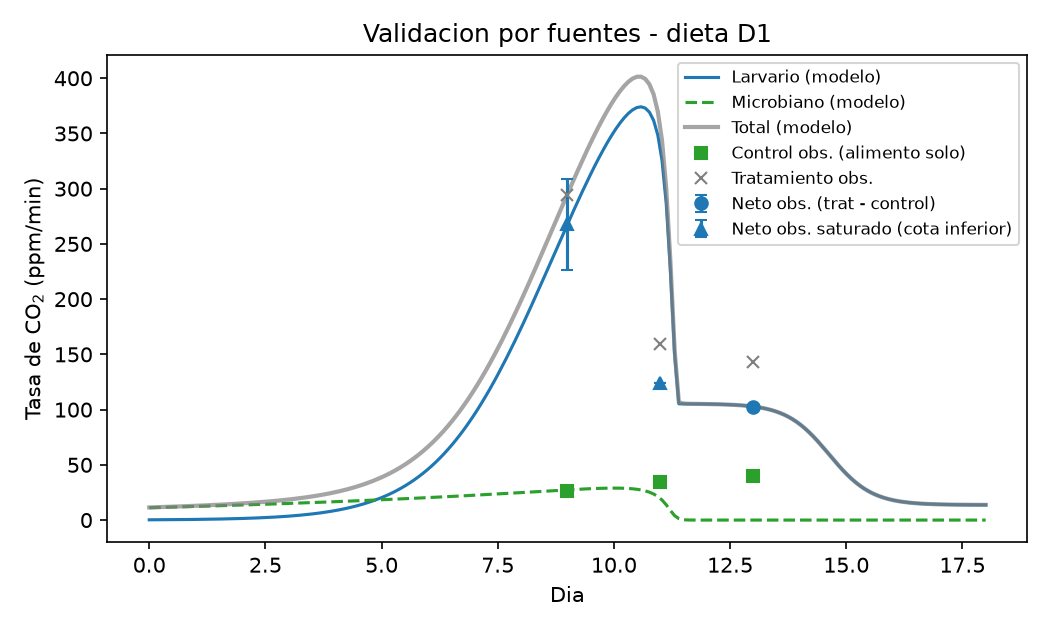
\includegraphics[width=0.85\textwidth]{figuras/validacion_co2_D1.png}
\caption{Validación por descomposición de fuentes, dieta D1 (alimento estándar). Curvas: componentes larvaria y microbiana y total del modelo para el régimen de carga única. Puntos: controles de alimento solo (cuadrados), tratamiento (x) y tasa neta tratamiento menos control (círculos; triángulos: cierres saturados, es decir cotas inferiores, con el rango entre cierres).}
\label{fig:valD1}
\end{figure}

\begin{figure}[htbp]
\centering
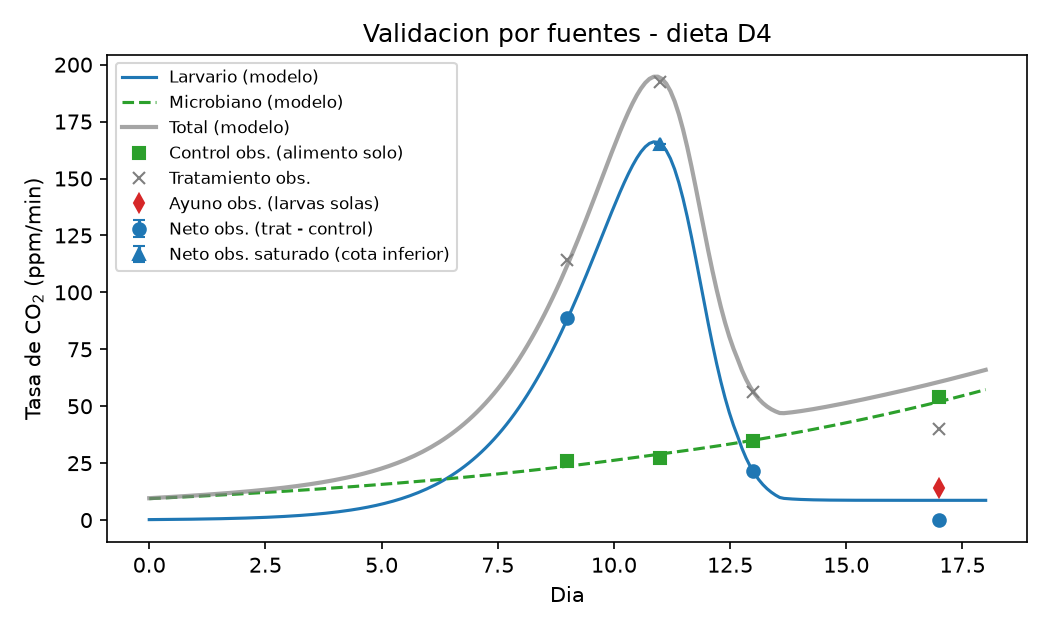
\includegraphics[width=0.85\textwidth]{figuras/validacion_co2_D4.png}
\caption{Validación por descomposición de fuentes, dieta D4 (residuos agroindustriales de frutas). Simbología como en la Figura \ref{fig:valD1}; el diamante es la tasa de larvas en ayuno medida el día 17.}
\label{fig:valD4}
\end{figure}

\paragraph{Nota sobre el CH$_4$.}
El canal de CH$_4$ (verificado en 0--10~\% en volumen) registró acumulaciones claramente medibles (pendientes de 300 a 3200~ppm/min, con $R^2 \geq 0.9$ en la mayoría de los cierres), pero sus dinámicas no fueron compatibles con la estructura del modelo: los controles de alimento solo decrecieron a lo largo del ciclo (de 1633 a 560~ppm/min en D1) mientras la degradación microbiana crece, los tratamientos no se separaron de forma consistente de sus controles (el día 9 midieron menos CH$_4$ que el control en ambas dietas) y aparecieron picos tardíos aislados (D4, día 17). Este patrón es atribuible a respuesta parcial del canal de CH$_4$ a volátiles de la fermentación del sustrato (etanol y otros compuestos orgánicos volátiles), y no a metanogénesis sola; por ello el término $\xi(\theta_s)$ del modelo se mantiene como indicador cualitativo de microambientes anóxicos y las lecturas de CH$_4$ se excluyeron de la validación cuantitativa; se retoma en la discusión.

\subsection{Análisis de sensibilidad}
Para evaluar cuánto dependen las conclusiones de los parámetros tomados de la literatura y del número aproximado de larvas, se recalibraron $B_0$, $f$, $t_p$ y $w_p$ perturbando uno a la vez $m$, $a_{\max}$ y $N$ en $\pm 20$~\% (Cuadro~\ref{tab:sensibilidad}). El ajuste es robusto al mantenimiento ($m$ $\pm 20$~\%: $R^2 \approx 0.98$ en D4, RMSE de 5.3 a 5.6 ppm/min), pero sensible a $a_{\max}$ y $N$: con $\pm 20$~\% el $R^2$ de D4 cae a $-2.44$ y $0.09$ ($a_{\max}$) y a $0.84$ y $0.93$ ($N$), y algunas cotas inferiores adicionales dejan de satisfacerse. La cota del día 11 de D1 queda incumplida en el caso base y en todos los escenarios de perturbación, lo que confirma su origen estructural (el agotamiento del sustrato en D1) y no un accidente de la calibración. Es decir, las tasas de gas sí restringen la combinación de parámetros: los valores cinéticos del núcleo DEB no son intercambiables, las conclusiones son condicionales a esos valores de la literatura y la sensibilidad cuantificada define la magnitud del riesgo, lo que refuerza la necesidad de una validación directa de biomasa que los fije de forma independiente.

\begin{table}[htbp]
\centering
\caption{Análisis de sensibilidad uno a la vez ($\pm 20$~\%) sobre los parámetros fijos $m$, $a_{\mathrm{máx}}$ y $N$, recalibrando $B_0$, $f$, $t_p$ y $w_p$ en cada caso. RMSE en ppm/min sobre los puntos no saturados (en D1, un solo punto); cotas D1/D4: margen porcentual mínimo sobre las cotas inferiores de los cierres saturados de cada dieta (negativo: cota violada).}
\label{tab:sensibilidad}
\begin{tabular}{lrrrrrrr}
\toprule
Perturbación & $B_0$ (mg) & $f$ (D4) & $R^2$ (D4) & RMSE (D4) & RMSE (D1) & cota D1 (\%) & cota D4 (\%) \\
\midrule
Base            & 0.0735 & 0.698 &  0.981 &  5.2 & 10.6 & $-25.9$ &  $-0.4$ \\
$m$ $-20$~\%    & 0.0656 & 0.705 &  0.980 &  5.3 & 10.7 & $-25.9$ &  $-1.9$ \\
$m$ $+20$~\%    & 0.0813 & 0.693 &  0.978 &  5.6 & 16.0 & $-25.8$ &    1.4  \\
$a_{\max}$ $-20$~\% & 0.278 & 0.730 & $-2.44$ & 69.9 &  9.9 & $-65.3$ & $-46.0$ \\
$a_{\max}$ $+20$~\% & 0.0136 & 0.722 & 0.086 & 36.1 & 11.9 & $-24.2$ & $-64.3$ \\
$N$ $-20$~\%    & 0.0924 & 0.711 &  0.840 & 15.1 & 10.5 & $-50.0$ &   21.6  \\
$N$ $+20$~\%    & 0.0515 & 0.707 &  0.933 &  9.8 & 10.8 & $-26.0$ & $-16.1$ \\
\bottomrule
\end{tabular}
\end{table}

\section{Discusion}
\label{sec:discusion}

(pendiente)

\section{Conclusiones}
\label{sec:conclusiones}

Se construyo y valido experimentalmente un modelo dinamico de emisiones de CO$_2$ en la bioconversion estatica con \textit{Hermetia illucens}, como extension del modelo DEB de Eriksen con tres componentes nuevos: un interruptor de prepupa, un modulo microbiano del lecho y el balance de gas de la camara estatica. La validacion por descomposicion de fuentes, con dos dietas y controles de alimento solo, mostro que la componente larvaria reproduce las tasas netas dentro de la incertidumbre experimental ($R^2 = 0.983$ y RMSE de 5.0 ppm/min en D4; cotas inferiores y punto limpio satisfechos en D1) y que el interruptor de prepupa es indispensable para capturar el colapso de las emisiones al final del ciclo. El ajuste permitio cuantificar, solo con mediciones de gas, la calidad relativa de la dieta de residuos ($f = 0.817$), los tiempos de prepupa por dieta y una biomasa inicial coherente con la postura de huevos, mientras que el modulo microbiano se calibro de forma independiente contra los controles ($k_{\mathrm{ref}} \approx 0.05$ d$^{-1}$, $Y_{CO_2} \approx 0.65$ a $0.69$). Las lecturas de CH$_4$ se mantuvieron como indicador cualitativo. Las extensiones futuras incluyen la validacion directa de biomasa, un estado de crecimiento microbiano y la incorporacion de O$_2$ y N$_2$O.


\printbibliography

\end{document}
